\documentclass[11pt]{article} % use larger type; default would be 10pt

\usepackage[utf8]{inputenc} % set input encoding (not needed with XeLaTeX)

\usepackage{geometry} % to change the page dimensions
\geometry{a4paper} % or letterpaper (US) or a5paper or....
% \geometry{margin=2in} % for example, change the margins to 2 inches all round
% \geometry{landscape} % set up the page for landscape
%   read geometry.pdf for detailed page layout information

\usepackage{graphicx} % support the \includegraphics command and options
\usepackage{authblk}
\usepackage{url}


\usepackage{caption}
\usepackage{subcaption}

% \usepackage[parfill]{parskip} % Activate to begin paragraphs with an empty line rather than an indent

%%% PACKAGES
\usepackage{booktabs} % for much better looking tables
\usepackage{array} % for better arrays (eg matrices) in maths
\usepackage{paralist} % very flexible & customisable lists (eg. enumerate/itemize, etc.)
\usepackage{verbatim} % adds environment for commenting out blocks of text & for better verbatim
\usepackage{subfig} % make it possible to include more than one captioned figure/table in a single float
% These packages are all incorporated in the memoir class to one degree or another...

\usepackage[polish]{babel}	
\usepackage{polski}
\usepackage[T1]{fontenc}
\frenchspacing	

\usepackage{indentfirst}

\usepackage{fancyhdr} % This should be set AFTER setting up the page geometry
\pagestyle{fancy} % options: empty , plain , fancy
\renewcommand{\headrulewidth}{0pt} % customise the layout...
\lhead{}\chead{}\rhead{}
\lfoot{}\cfoot{\thepage}\rfoot{}

%%% SECTION TITLE APPEARANCE
\usepackage{sectsty}
\allsectionsfont{\sffamily\mdseries\upshape} % (See the fntguide.pdf for font help)
% (This matches ConTeXt defaults)

%%% ToC (table of contents) APPEARANCE
\usepackage[nottoc,notlof,notlot]{tocbibind} % Put the bibliography in the ToC
\usepackage[titles,subfigure]{tocloft} % Alter the style of the Table of Contents
\renewcommand{\cftsecfont}{\rmfamily\mdseries\upshape}
\renewcommand{\cftsecpagefont}{\rmfamily\mdseries\upshape} % No bold!

%%% END Article customizations

%%% The "real" document content comes below...

\title{San Francisco Crime Classification\\ \large{Kaggle competition  }}
\author{Łukasz Rados, Wojciech Kusa}

\affil{Wydział Fizyki i Informatyki Stosowanej \\ Akademia Górniczo-Hutnicza w Krakowie}


%\date{} % Activate to display a given date or no date (if empty),
         % otherwise the current date is printed 

\begin{document}
\maketitle

\section{Wprowadzenie}

Celem projektu było stworzenie oprogramowania pozwalającego dokonać klasyfikacji zgłoszeń na podstawie danych czasoprzestrzennych z raportów policyjnych dla miasta San Francisco w Stanach Zjednoczonych. Pełen opis projektu, wraz z danymi wejściowymi znajduje się na portalu kaggle, pod adresem: \url{www.kaggle.com/c/sf-crime/}.


\section{Dane} \label{sec:data}

Zbiór danych zawiera incydenty zgłoszone policji w San Francisco pomiędzy 01.01.2003r. a 13.05.2015r.. Podzielony jest na dwie podgrupy (prawie równoliczne, w każdej po około 850 tysięcy elementów) :
\begin{itemize}
\item zbiór treningowy -- zawierający zgłoszenia z tygodni parzystych,

\item zbiór testowy --  zawierający zgłoszenia z tygodni nieparzystych.
\end{itemize} 

Przykładowe wiersze danych treningowych znajdują się na Rysunku \ref{fig:train_data}. Dane składają się z następujących pól:

\begin{itemize}
\item Dates -- znacznik czasu przestępstwa
\item DayOfWeek -- dzień tygodnia
\item PdDistrict -- nazwa departamentu policji odbierającego zgłoszenie
\item Address -- przybliżony adres przestępstwa
\item X -- długość geograficzna
\item Y -- szerokość geograficzna
\item Category -- kategoria przestępstwa (tylko dla zbioru treingowego). Jest to zmienna, którą należało przewidzieć w wyniku działania algorytmu
\item Descript -- szczegółowy opis przestępstwa (tylko dla zbioru treingowego)
\item Resolution -- jaki był wynik działania policji (tylko dla zbioru treingowego)

\end{itemize}

\begin{figure}[!h]
  \centering
    \includegraphics[width=0.95\textwidth]{images/train_data.png}
  \caption{Przykładowe dane treningowe. Źródło: \protect\url{https://www.kaggle.com/c/sf-crime/data} } \label{fig:train_data}
\end{figure}



\subsection{Wstępna analiza zbioru treningowego}

Zbiór treningowy zawiera ponad 878 tys. zgłoszeń z okresu od 1 stycznia 2003r. do 13 maja 2015r. Przestępstwa pogrupowane zostały na 39 kategorii, których liczności przedstawiono na Rysunku \ref{fig:categories}. Większość zdarzeń zaliczona została do kategorii \textit{Larency / Theft} (ang. kradzież), \textit{Assault} (ang. napaść) i \textit{Drug / Narcotic} (ang. narkotyki) oraz grup gromadzących pozostałe zdarzenia (\textit{Non-Criminal} oraz \textit{Other Offences}).  \\

\begin{figure}[!h]
  \centering
    \includegraphics[width=0.95\textwidth]{images/categories}
  \caption{Zgłoszenia podzielone według przypisanej kategorii.} \label{fig:categories}
\end{figure}

Podczas analizy zbioru danych znaleziono silną zależność pomiędzy godziną a liczbą przestępstw: najmniej zgłoszeń odnotowano w godzinach 3:00 -- 7:00, zaś najniebezpieczniejsze są godziny 15:00 -- 20:00 (Rysunek \ref{fig:hours}). Ponadto zauważono, że rozkład zgłoszeń w czasie różni się w zależności od wybranej kategorii. Przykładem mogą być rozkłady godzinne zgłoszeń związanych z prowadzeniem po spożyciu alkoholu oraz przestępstwa narkotykowe: te pierwsze zdarzają się głównie pomiędzy godziną 20:00 a 3:00, zaś te drugie pomiędzy 12:00 a 20:00. W związku z tym prawdopodobieństwo, że przestępstwo popełnione około godziny 16 jest związane z alkoholem jest dużo mniejsze, niż szansa jego związku z narkotykami. Na Rysunkach \ref{fig:crimes_per_hour_1} -- \ref{fig:crimes_per_hour_6} przedstawiono sześć przykładowych rozkładów.  \\

\begin{figure}[!h]
  \centering
    \includegraphics[width=0.95\textwidth]{images/hours}
  \caption{Zgłoszenia podzielone według godziny w ciągu dnia.} \label{fig:hours}
\end{figure}


\begin{figure}[!h]
\centering
   \begin{subfigure}{0.48\linewidth}
   \centering
   \includegraphics[width=\linewidth]{images/crimes_per_hour/6}
   \caption{Prowadzenie pod wpływem alkoholu}
   \label{fig:crimes_per_hour_1} 
\end{subfigure}
\hfill
\begin{subfigure}{0.48\linewidth}
   \centering
   \includegraphics[width=\linewidth]{images/crimes_per_hour/1}
   \caption{Napad}
   \label{fig:crimes_per_hour_2}
\end{subfigure}
\\[\baselineskip]
\begin{subfigure}{0.48\linewidth}
   \centering
   \includegraphics[width=\linewidth]{images/crimes_per_hour/7}
   \caption{Narkotyki}
   \label{fig:crimes_per_hour_3}
\end{subfigure}
\hfill
\begin{subfigure}{0.48\linewidth}
   \centering
   \includegraphics[width=\linewidth]{images/crimes_per_hour/8}
   \caption{Pijaństwo}
   \label{fig:crimes_per_hour_4}
\end{subfigure}
\\[\baselineskip]
   \begin{subfigure}{0.48\linewidth}
   \centering
   \includegraphics[width=\linewidth]{images/crimes_per_hour/16}
   \caption{Kradzież}
   \label{fig:crimes_per_hour_5} 
\end{subfigure}
\hfill
\begin{subfigure}{0.48\linewidth}
   \centering
   \includegraphics[width=\linewidth]{images/crimes_per_hour/12}
   \caption{Fałszerstwo}
   \label{fig:crimes_per_hour_6}
\end{subfigure}
\centering
\caption{Przykładowe zależności pomiędzy liczbą zgłoszeń a godziną.} 
\end{figure}

Na podstawie kolumny \textit{Address} (zawierającej przybliżony adres zgłoszenia) ustalono, czy wykroczenie miało miejsce na skrzyżowaniu dwóch ulic. Okazuje się, że niektóre z przestępstw (podejrzane zachowanie, prostytucja, jazda pod wpływem alkoholu czy sprzedaż narkotyków) są zazwyczaj powiązane ze skrzyżowaniami (w przypadku prostytucji około 80\% zanotowanych przypadków miało miejsce na skrzyżowaniach). Wysoki odsetek zatrzymań za jazdę pod wpływem alkoholu na rogu ulic związany jest zapewne z rozmieszczeniem patroli policyjnych. Dane dla wszystkich przestępstw zamieszczono na wykresie \ref{fig:corner}. \\

\begin{figure}[!h]
  \centering
    \includegraphics[width=0.95\textwidth]{images/street_corner}
  \caption{Odsetek wykroczeń popełnianych na skrzyżowaniach do ogólnej liczby wykroczeń w danej kategorii.} \label{fig:corner}
\end{figure}

Na rysunku \ref{fig:sf_districts} znajduje się mapa San Francisco z zaznaczpnymi wszystkimi przestępstami podzielonymi ze względu na posterunek odbierający zgłoszenie. \\

W trakcie analizy zbioru uczącego i przygotowywania wykresów, zauważono kilka ciekawych (chociaż niezwiązanych z tematem pracy) zależności. Niektóre z nich przytoczono poniżej:

\begin{itemize}
\item Około 80\% przypadków prostytucji miało miejsce na skrzyżowaniach (rysunek \ref{fig:corner}), co więcej -- większość przypadków prosytucji odnotowano w dwóch skupiskach (rysunek \ref{fig:sf_crimes_prostitution});
\item Włamania są najczęstsze w godzinach 9 - 18 (wtedy, gdy większość osób jest w pracy);
\item Zatrzymania związane ze spożyciem alkoholu zaczynają się pojawiać od godziny 6 rano i rosną systematycznie aż do północy;
\item Największa część przypadków agresji domowej notowana jest w godzinach 13 - 15, co może być związane z końcem tzw. pierwszej zmiany;
\item Kradzieże kieszonkowe mają miejsce głównie w okolicach godzin szczytu (16 - 18);
\item Samochody są najczęściej kradzione między 18 a 22, zaś odzyskiwane -- w godzinach południowych;
\item Na 53781 zgłoszonych kradzieży samochodu przypada tylko 3138 odzyskanych pojazdów (około 6\%).
\end{itemize}

Zauważone zależności pozwalają przypuszczać, że między poszczególnymi atrybutami kolejnych rekordów, zidentyfikować można subtelne powiązania. \\


\subsection{Zastosowane deskryptory}

Wstępna analiza zbioru treningowego pozwoliła wykluczyć z dalszej pracy następujące kolumny: \textit{Address} (z którego wyciągnięto tylko informację o skrzyżowaniu), \textit{Dates} (podzielono na rok, miesiąc, godzinę i minutę dnia), \textit{Resolution} oraz \textit{Descript} (kolumny zawierają w żaden sposób nieusystematyzowany tekst). \\

Dane poddane zostały preprocessingowi celem poprawy brakujących rekordów, a następnie, poza podstawowymi zmiennymi przedstawionymi w sekcji \ref{sec:data}, przygotowano dodatkowe deskryptory mające pomóc wytrenować model. Poniżej zostały opisane najważniejsze z nich, mające istotny wpływ na poprawę działania modelu:

\begin{itemize}
\item $Dates.Hours \cdot 60 + Dates.Minutes$ - Liczba z zakreu {0, 1440} opisująca, w której minucie dnia zostało dokonane zgłoszenie

\item $X \cdot Y$ - wskazuje na nieliniową korelację długości i szerokości geograficznej

\item $X + Y$ - jak wyżej, zmienna wskazująca na korelację długości i szerokości geograficznej

\item informacja czy przestępstwo zostało dokonane na skrzyżowaniu / rogu ulicy - wyciągnięta ze zmiennej Address

\item informacja czy przestępstwo zostało dokonane w bloku - wyciągnięta ze zmiennej Address

\item $DayOfWeek + Dates.Hour$  - powiązuje godzinę zdarzenia z dniem tygodnia

\item $DayOfWeek \cdot Dates.Hour$ -  jak wyżej, powiązuje godzinę zdarzenia z dniem tygodnia

\end{itemize}

\begin{figure}[!h]
\centering
   \begin{subfigure}{0.48\linewidth}
   \centering
   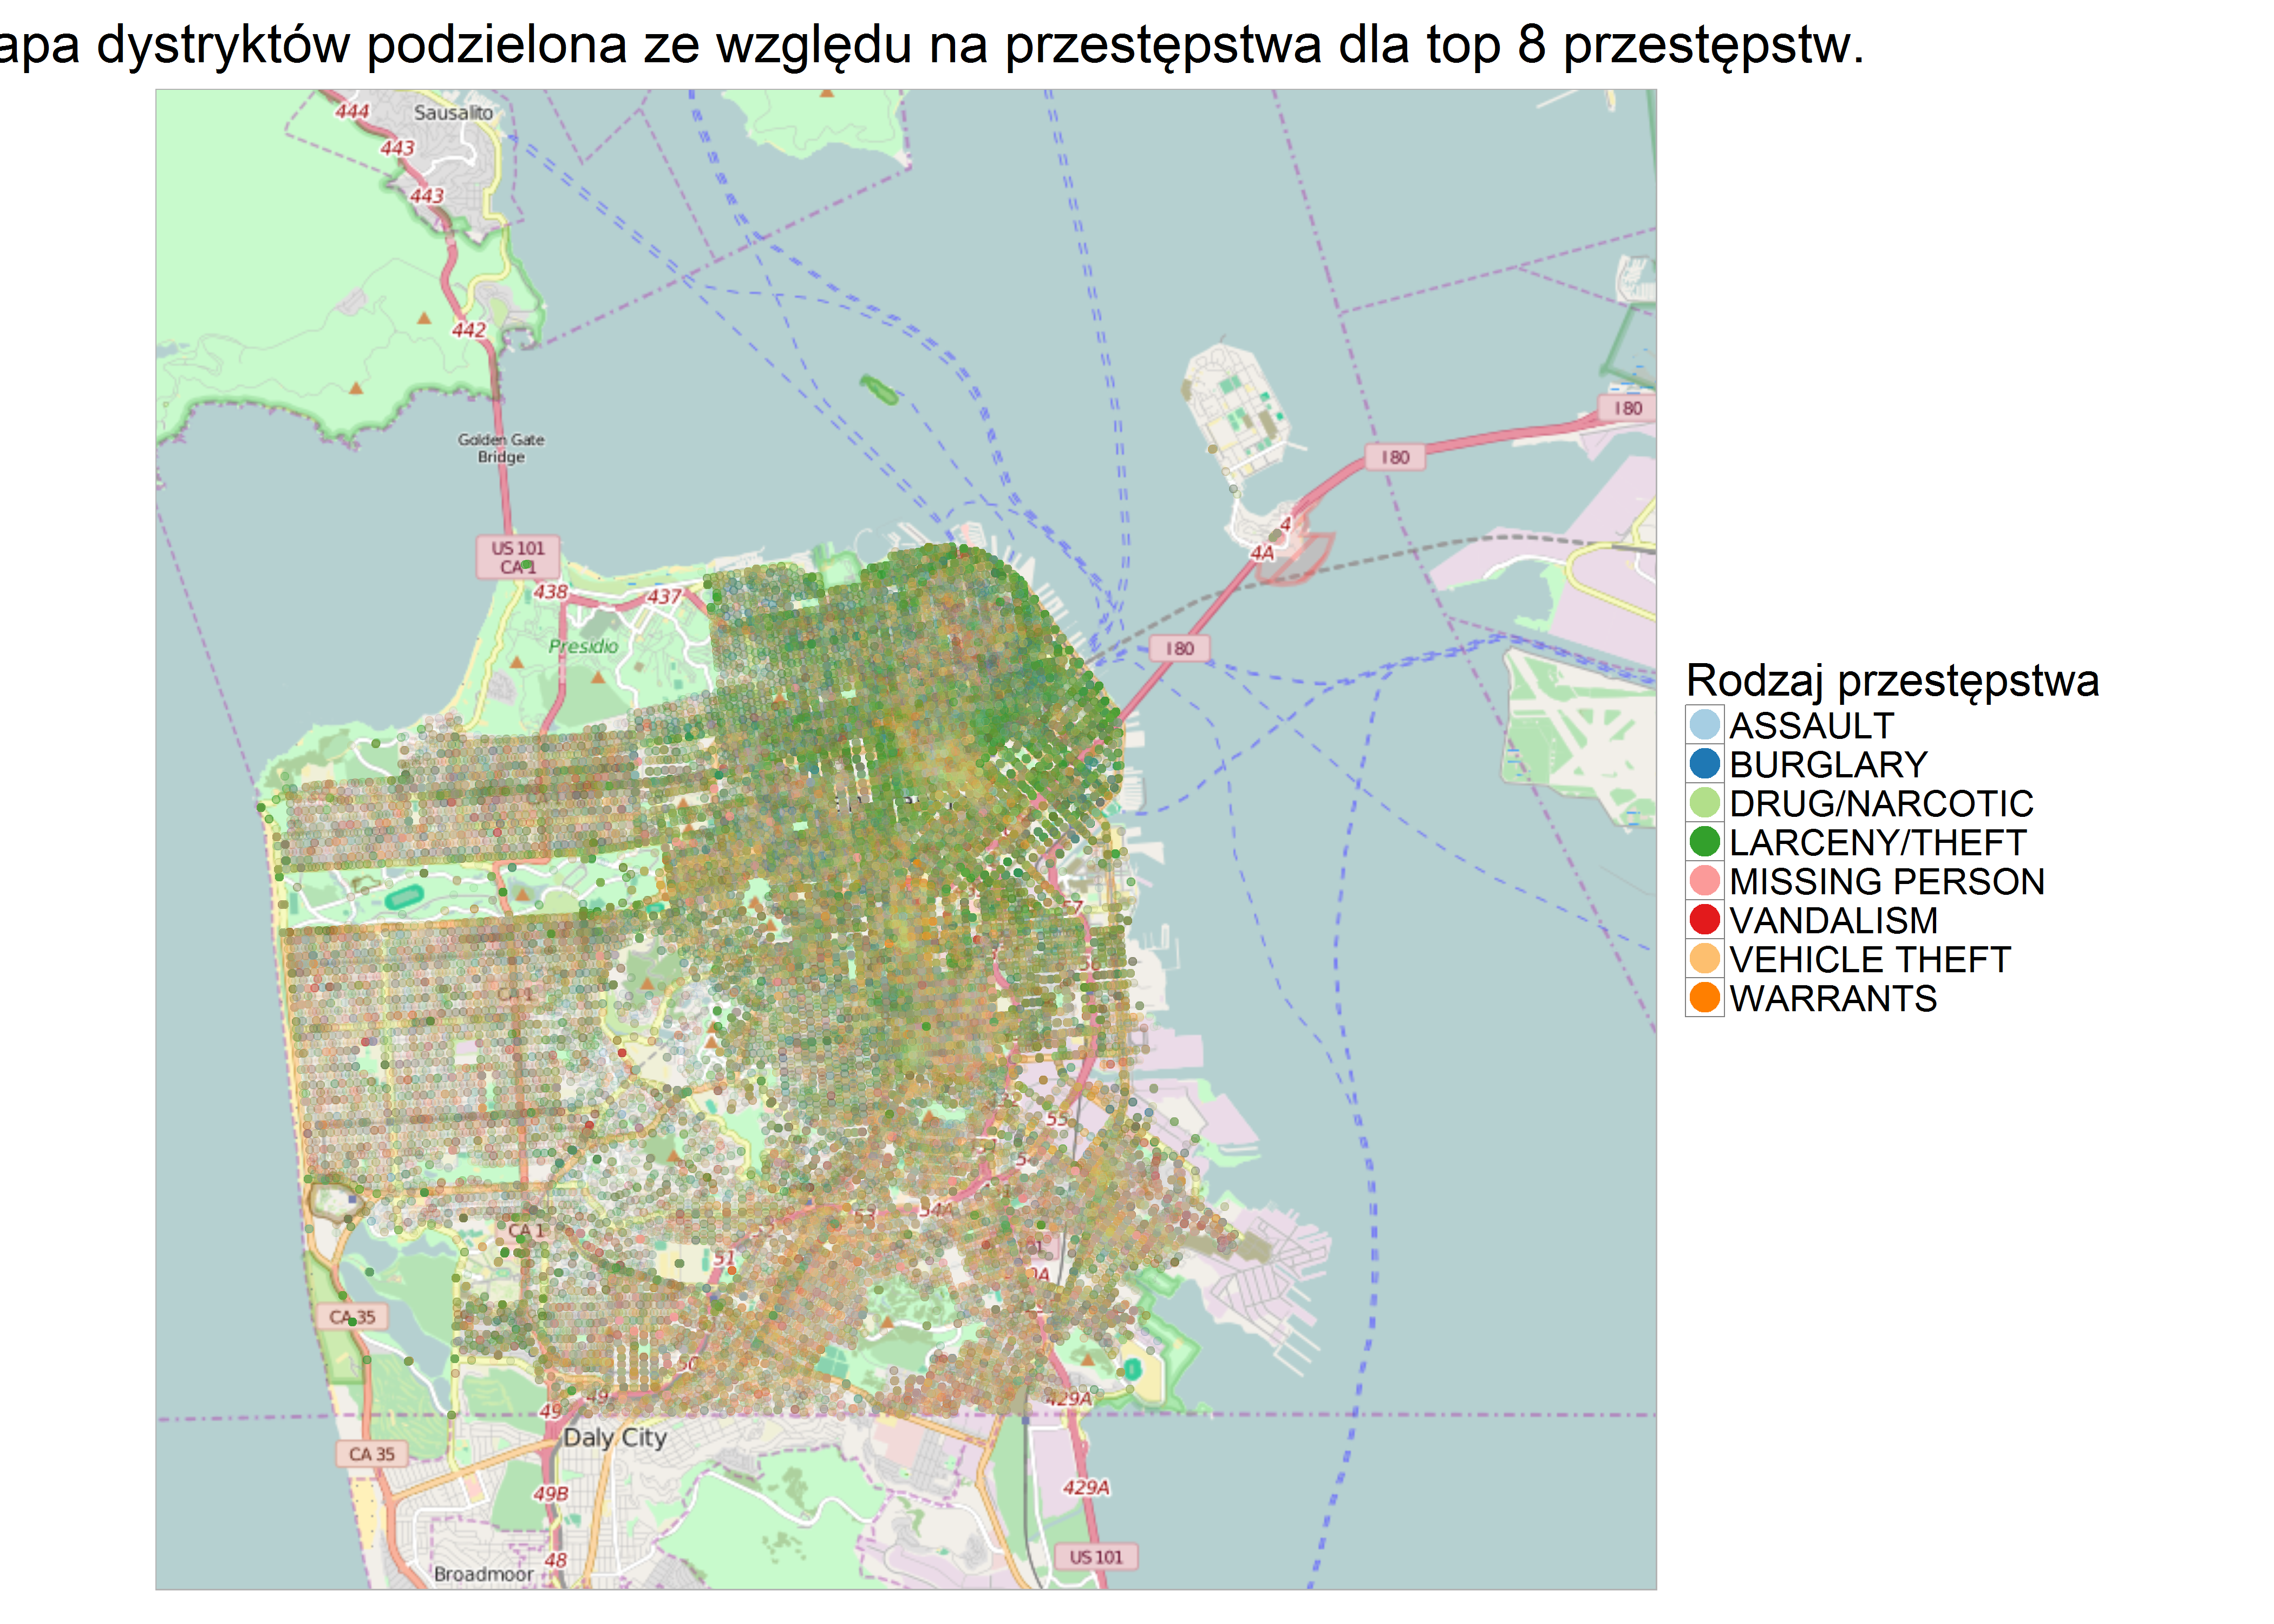
\includegraphics[width=\linewidth]{images/sf_crimes_all}
   \caption{Mapa San Francisco z naniesionymi 8 najliczniejszymi rodzajami zgłoszeń. W przypadku wyświetlenia wszystkich rodzajów przestępstw, otrzymano w praktyce różnokolorową mozaikę, bardzo trudną do interpretacji.}
   \label{fig:sf_top8} 
\end{subfigure}
\hfill
\begin{subfigure}{0.48\linewidth}
   \centering
   \includegraphics[width=\linewidth]{images/sf_districts}
   \caption{Przestępstwa podzielone ze względu na posterunek odbierający zgłoszenie.} 
   \label{fig:sf_districts}
\end{subfigure}
\\[\baselineskip]
   \begin{subfigure}{0.48\linewidth}
   \centering
   \includegraphics[width=\linewidth]{images/sf_crimes_3}
   \caption{Wyraźnie widoczna kumulacja przypadków prostytucji w dwóch miejscach w mieście (pozostałe kategorie rozkładają się mniej więcej równomiernie na całej mapie).}
   \label{fig:sf_crimes_prostitution} 
\end{subfigure}
\hfill
\begin{subfigure}{0.48\linewidth}
   \centering
   \includegraphics[width=\linewidth]{images/sf_crimes_4}
   \caption{Jeden z nielicznych przypadków korelacji widocznej na podstawie mapy: powiązanie przestępstw narkotykowych z wymuszeniami seksualnymi.}
   \label{fig:sf_crimes_drugs}
\end{subfigure}
\centering
\caption{Dane treningowe naniesione na mapę San Francisco.}
\end{figure}

\clearpage

\section{Zastosowane algorytmy}
\subsection{Lasy losowe - Random Forest}

Algorytm Lasów Losowych (ang. \textit{Random Forest Algorithm, RF}) to metoda klasyfikacji oparta na koncepcji bagging (podział zadania na podzbiory złożone z losowo wybranych rekordów zbioru treningowego, każdy podzbiór analizowany jest przez niezależnego eksperta. Wyniki otrzymuje się w wyniki głosowania ekspertów). Spośród całego zbioru treningowego $D$ wybieranych jest $N$ podzbiorów, każdy o rozmiarze $m$ (gdzie $m$ jest mniejsze od rozmiaru zbioru treningowego). Dla każdego z podzbiorów tworzone jest drzewo decyzyjne (algorytm korzysta więc z $N$ drzew decyzyjnych). Ostateczna wynik klasyfikacji otrzymywany jest poprzez wybranie klasy zwróconej przez największą liczbę drzew.\\

Do zalet algorytmu zaliczyć można jego skalowalność (w miarę dostępności pamięci operacyjnej), małe prawdopodobieństwo przeuczenia oraz prostotę implementacji. W programie wykorzystano implementację algorytmu dostępną w bibliotece sklearn.


\subsection{Generalized Linear Model}

Uogólniony model liniowy (ang. \textit{Generalized Linear Model, GLM}) jest rozszerzeniem zwykłej regresji liniowej pozwalającej na modelowanie zmiennych posiadających inny niż normalny rozkład błędu. GLM zezwala aby model liniowy był skorelowany z odpowiedzią poprzez funkcję łączącą (ang. \textit{link function}) oraz wielkość wariancji dla każdego pomiaru być funkcją jego przewidywanej wartości. \\

Do klasyfikacji przestępstw wybrano dwumianowy rozkład błędu liczący ilość wystąpień danego przestępstwa na zasadzie binarnej {tak, nie}. Jako link function zastosowano funkcję logitową. \\

\section{Implementacja}

Kody źródłowe zaimplementowanych modeli znajdują się w repozytorium on-line pod adresem \url{www.github.com/WojciechKusa/sf_crime}. 

\subsection{Lasy losowe - Random Forest}

Model wykorzystujący algorytm Lasów Losowych zaimplementowany został w języku programowania Python z wykorzystaniem biblitek pandas, sklearn oraz seaborn (do wizualizacji). Ze względu na ograniczone zasoby sprzętowe (program uruchamiany był na komputerze z 8Gb pamięci RAM), liczność lasu została ustalona na poziomie 52 drzew. Większa liczba drzew zapewne pozwoliłaby na osiągnięcie lepszego wyniku (choć wątpliwe, by była to poprawa rzędu większego niż 0.1). W modelu uwzględniono następujące zmienne:

\begin{itemize}
\item $PdDistrict$
\item $X $
\item $Y $
\item $DayOfWeek$
\item $Dates.Year $
\item $Dates.Month $
\item $Dates.Hours $
\item $Dates.Hours \cdot 60 + Dates.Minutes$ 
\item $Block $ -- informacja (0/1) czy wydarzenie miało miejsce w bloku
\item $Corner $ -- informacja (0/1) czy wydarzenie miało miejsce na skrzyżowaniu
\end{itemize}

\subsection{Generalized Linear Model}

Model wykorzystujący GLM zaimplementowany został w języku R z wykorzystaniem bibliotek MASS, readr, rpart oraz caret. Do ostatecznego modelu wzięte zostały następujące zmienne:

\begin{itemize}
\item $PdDistrict$
\item $X $
\item $Y $
\item $X \cdot Y$
\item $X + Y$ 
\item $DayOfWeek$
\item $Dates.Year $
\item $Dates.Month $
\item $Dates.Hours $
\item $Dates.Hours \cdot 60 + Dates.Minutes$ 
\item $DayOfWeek + Dates.Hour $
\item $DayOfWeek \cdot Dates.Hour $
\item $AddressType $ -- informacja czy zdarzenie miało miejsce na skrzyżowniu czy w bloku

\end{itemize}


\section{Ewaluacja oraz wyniki}

\subsection{Ocena modeli}

Ocena modeli dokonywana była na podstawie wielo-klasowej straty logarytmicznej (ang. \textit{multi-class logarithmic loss}). Dane zawierały prawdopodobieństwa wystąpienia danego przestępstwa przy podanych danych czasoprzestrzennych. \\

\subsection{Uzyskane wyniki}


W przypadku zastosowania modelu GLM uzyskany wynik to 2.51443 punkta co na dzień 24.01.2016r. dało 267 miejsce na około 1200 uczestników. Dla modelu RF otrzymano wynik 5.70246 co plasuje go na 889 miejscu. Wyniki te można uznać za satysfakcjonujące gdy weźmie się pod uwagę fakt, że najlepszy aktualnie wynik to 2.05079 a pierwsze 900 rezultatów to wyniki poniżej 10 punktów. Wynik dla rozwiązania losowego to 26 punktów. \\


\section{Podsumowanie}

Zadanie \textit{San Francisco Crime Classification} nie należy do łatwych -- już sama analiza mapy \ref{fig:sf_top8} pozwala stwierdzić, że już dla 8 najczęściej raportowanych incydentów operowanie na danych czasoprzestrzennych jest trudne. Wyniki pierwszych 100 zawodników dzielą dziesiąte części punktów, co świadczy o dużej i wyrównanej rywalizacji. Konkurs uruchomiony został 2 czerwca 2015 roku, co oznacza że zespoły biorące w nim udział miały ponad pół roku na dopracowanie swoich rozwiązań. \\

W tym kontekście, dla zastosowanych modeli GLM i RF uzyskano satysfakcjonujące rezultaty. Potwierdzają to wyniki w systemie konkursowym plasujące modele odpowiednio w top 300 oraz top 900 z wynikami punktowymi niewiele odstającymi od najlepszych rezultatów. \\

Dalszym rozwojem algorytmów mogłoby być stworzenie rozkładów gęstości prawdopodobieństwa i poszukanie korelacji pomiędzy przestępstwami co pozwoliłoby związać kilka zmiennych i (być może) uprościć model odpowiedzialny za predykcję z 39 zmiennych. Ponadto ciekawym i wartym przetestowania rozwiązaniem mogłoby być faworyzowanie częściej powtarzających się przestępstw a zerowanie prawdopodobieństwa dla tych rzadko występujących. \\

W przypadku rozwiązania napisanego w Pythonie, warto byłoby sprawdzić zachowanie algorytmu dla lasu złożonego z większej liczby drzew (np. 500 zamiast używanych 52). \\

\end{document}
